\documentclass[fleqn,a4paper,12pt]{article}

%used Packages
\usepackage{standalone}		% Zum Einlesen aus anderen .tex-Files
\usepackage{geometry}		% Zur Bearbeitung des Layouts (Ränder,...)
\usepackage[german]{babel}
\usepackage[utf8]{inputenc}
\usepackage{amsmath}		% Mathematische Symbole
\usepackage{amssymb}     	% Nochmehr mathematische Symbole
\usepackage{dsfont}      	% Schriftsatz fuer Zahlenmengensymbole
%\usepackage{verbatim}   	% erweiterte Verbatim-Umgebung
\usepackage{alltt}       	% Quasi-Verbatim-Umgebung
\usepackage{fancyhdr}    	% Eigene Kopfzeilen
\usepackage{graphicx}    	% Zum Einbinden von Grafiken
							% Einbinden einer eps-Grafik geht so: includegraphics{path}
\usepackage{wrapfig}
\usepackage{lscape}
\usepackage{rotating}
\usepackage{epstopdf}

% Skalierung der Grafiken
\setlength{\unitlength}{1cm}

\frenchspacing               % Kein Extrafreiraum nach Satzzeichen
\setlength{\parindent}{0pt}  % Neue Absaetze nicht einruecken
%\sloppy                     % Schlampige Absatzformatierung
\fussy                       % Penible Absatzformatierung
\linespread{1.5}             % Zeilenabstand


% Seitenraender
\geometry{left=30mm, right=40mm, bottom=30mm}
				% Doc-class, Packageimports, fancy stuff
%Seitenränder formatieren
\addtolength{\voffset}{-2cm}
\addtolength{\textheight}{0cm}
\addtolength{\hoffset}{0cm}
\addtolength{\textwidth}{2cm}
\addtolength{\headheight}{2cm} % fuer jeden Strichkode einen Zentimeter

% Font fuer Code 39
\font\xlix=wlc39 scaled 1200
\newcommand\barcode[1]{{\xlix@#1@}}

% Name, Matrikelnummer, Barcode
\newcommand\student[2]{
	\mbox{\scriptsize
		\begin{tabular}{@{}l@{}r@{}}
			\multicolumn{2}{@{}r@{}}{\barcode{#2}}\\
			#1&#2\\
		\end{tabular}}}

% Kopfzeile
\pagestyle{fancy}            % Eigene Kopfzeilen verwenden
\lhead{
	\small
	\textsc{Grundlagen der Signalverarbeitung \\
		WS 2017/2018 \\
		\"Ubung (\today)}
	\vfill}
\rhead{
	\begin{tabular}[b]{@{}rr@{}}
		\student{Philipp Badenhoop}{572693} &
		\student{Steven Lange}{568733} \\
		\student{Pascal Jochmann}{575056} &
		\student{Kevin Trogant}{572451}
\end{tabular}}			% Definition der Kopfzeile
%andere Definitionen
\providecommand{\R}{{\mathbb R}}
\providecommand{\N}{{\mathbb N}}
\providecommand{\Z}{{\mathbb Z}}
\providecommand{\Q}{{\mathbb Q}}
\providecommand{\C}{{\mathbb C}}
\providecommand{\F}{\mathcal{F}}
\providecommand{\less}{\setminus}
\providecommand{\inv}{{}^{-1}}
\providecommand{\Land}{\bigwedge}
\providecommand{\Lor}{\bigvee}			% Liste der zusätzlichen Commands und redefines

\begin{document}
	\section*{Übungsaufgabe 29:}
		Sei $f(t) = 3t\cdot e^{-2t}, t\ge 0$.\\
		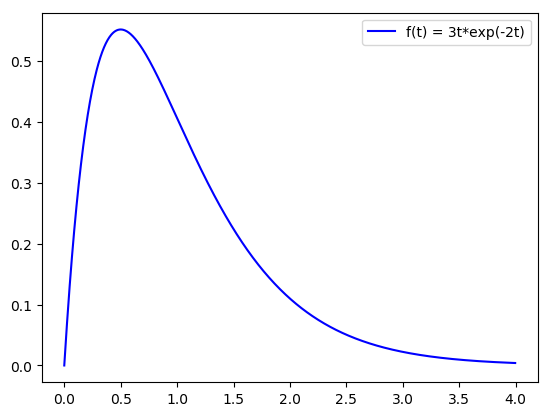
\includegraphics[scale = 0.7]{A29_graphPlot.png}\\
		\\
		Sei weiter $g(t) = t\cdot e^{-2t}, t\ge 0$ und $h(t)=e^{-2t}, t\ge 0$.\\
		Da der Faktor $t$ in der Transformierten $F(\omega)$ nicht mehr auftaucht, ist die Transformierte von $f(t)$ der von Aufgabe 29 ähnlich. Insbesondere wird $F(\omega)$ durch den Faktor 3 gestreckt. Daher gilt die Schätzung: $F(0) = 3$\\
		Dann gilt:
		$$ f(t) = 3\cdot g(t) = 3t \cdot h(t),\quad t\ge 0$$
		Dann gilt nach den tabellierten Fouriertransformierten vom Arbeitsblatt das folgende:\\
		\begin{tabular}{c | c | l | l}
			Zeile	&	 Name	&	Signal			&	Fouiertransformierte\\
			\hline
			1		&	$f(t)$	&	$3 \cdot g(t)$	&	$3\cdot G(\omega)$\\
			5		&	$g(t)$	&	$t \cdot h(t)$	&	$j\cdot \frac{d}{d\omega}H(\omega)$\\
			D		&	$h(t)$	&	$e^{-t}$		&	$\frac{1}{1+j\omega}$
		\end{tabular}\\
		Das heißt für die Fouiertransformierte $F(\omega)$ gilt:
		$$F(\omega) = 3\cdot \left(j\cdot \frac{d}{d\omega}\left(1+j\omega\right)^{-1}\right) = 3\left(-\left(1+j\omega\right)^{-2}\cdot j^2\right) = \frac{3}{(1+jw)^2}$$
		\newpage
		Mit folgenden Graphen:\\
		\textbf{Plot des Real- (blau) und Imaginäranteils (rot):}\\
		\includegraphics[width = 0.85\textwidth]{A29_plot-real-imag.png}\\
		\textbf{Plot des Betrags (blau) und des Winkels (rot) in [$\pi$]:}\\
		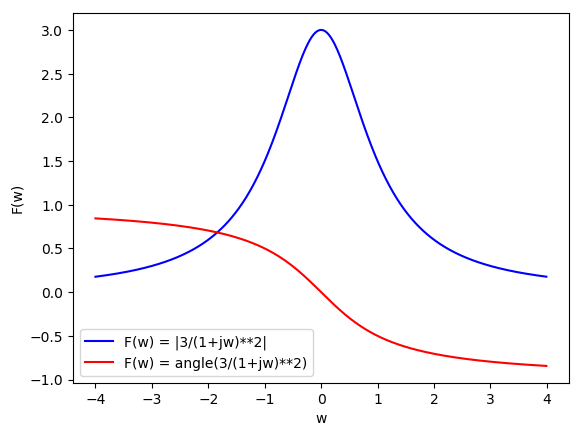
\includegraphics[width= 0.85\textwidth]{A29_plot-abs-angle.png}\\
		\textbf{Niquest-Plot von $F(\omega)$ mit $\omega\in[-4,4]$:}\\
		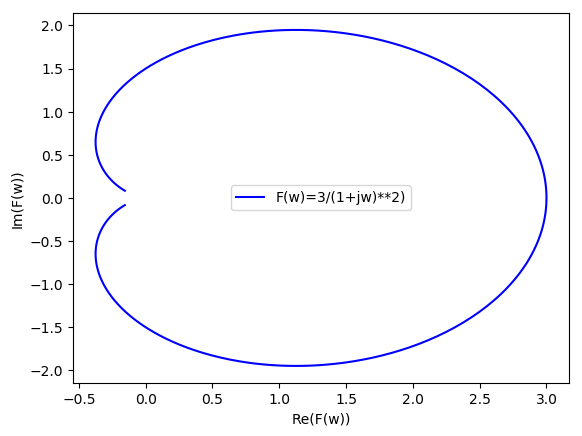
\includegraphics[width=\textwidth]{A29_niquest-plot.png}
\newpage
	\section*{Übungsaufgabe 30:}
		Sei $f(t) = 3t\cdot e^{-2t}, t\ge 0$.
        Als diskrete Funktion mit Abtastintervall $T_A = \frac{1}{8}$, mit $N = 64$ Samples, wählen wir: $f_n = f(n \cdot T_A)$. \\
        \includegraphics[width=\textwidth]{A30_Fn.png} \\
        Nach der diskreten Fourier-Transformation ergibt sich folgendes Betragsspektrum: \\
        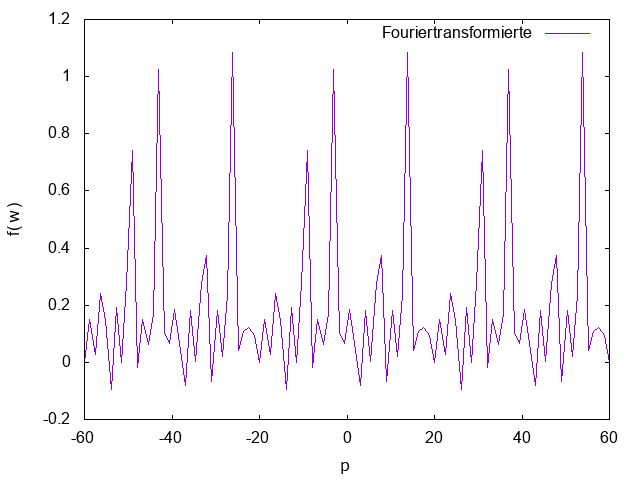
\includegraphics[width=\textwidth]{A30_Abs.png}
\newpage\end{document}